\documentclass[11pt]{article}
\usepackage{latexsym,amssymb,amsthm,amsmath,bbm,graphicx,float,cite,color,wasysym,widetable,subcaption}

\pdfpagewidth 8.5in
\pdfpageheight 11in
\topmargin 0in
\textheight 8.5in
\textwidth 6.5in
\oddsidemargin 0in
\evensidemargin 0in

\newcommand{\R}{\mathbb{R}}
\newcommand{\E}{\mathbb{E}}
\newcommand{\Var}{\operatorname{Var}}
\newcommand{\tr}{\operatorname{tr}}
\newcommand{\diag}{\operatorname{diag}}
\newtheorem{definition}{Definition}

\begin{document}
\title{1D Experiment}
\author{Kun Dong}
\date{Mar 22nd, 2017}
\maketitle

\section{Setup}
In this experiment, we set the Hamiltonian operator $H = -\frac{1}{2}L +V$ on the interval $[0,20]$, where $L$ is the Laplacian operator with periodic boundary condition, and $V$ is the sum of $7$ Gaussians distributions (one at each end and $5$ chosen uniformly random). After discretization the interval into $n$ points, we take the first $N$ eigenvectors as the orbits. The relative error is measured as $\|\widetilde{\rho}-\rho\|_F/\|\rho\|_F$. Due to randomness in $V$, we do $10$ different runs and show the averaged results below.

\section{Comparing QRSC and Voronoi}
\begin{table}[H]
	\begin{widetable}{\textwidth}{c c| c c c |c c c}
	\hline
		&  & \multicolumn{3}{|c}{QRSC} & \multicolumn{3}{|c}{Voronoi}\\
	\hline
	$N$ & $n$ & $N_{aux}$ & rel-err & time(s) & $N_{aux}$ & rel-err & time(s)\\
	\hline\hline
	$100$ & $1024$ & $198$ & 1.18E-6 $\pm$ 4.61E-7 & $1.764$ & $400$ & 1.00E-6 $\pm$ 1.26E-6 & $0.187$\\
	$200$ & $1024$ & $406$ & 1.39E-6 $\pm$ 5.77E-7 & $4.387$ & $792$ & 1.66E-6 $\pm$ 1.06E-6 & $1.176$ \\
	$300$ & $1024$ & $608$ & 1.91E-6 $\pm$ 3.64E-7 & $9.115$ & $952$ & 1.24E-6 $\pm$ 2.16E-7 & $3.406$\\
	\hline
	$100$ & $2048$ & $198$ & 4.71E-7 $\pm$ 3.59E-7 & $4.993$ & $400$ & 3.57E-7 $\pm$ 3.44E-7 & $0.674$\\
	$200$ & $2048$ & $397$ & 4.98E-7 $\pm$ 1.83E-7 & $12.391$ & $800$ & 2.32E-7 $\pm$ 8.11E-8 & $2.145$\\
	$300$ & $2048$ & $601$ & 1.24E-6 $\pm$ 6.57E-7& $25.132$ & $1200$ & 2.57E-6 $\pm$ 4.48E-6 & $10.809$\\
	\hline
	$100$ & $4096$ & $198$ & 4.03E-7 $\pm$ 4.04E-7 & $10.897$ & $400$ & 4.08E-7 $\pm$ 6.94E-7 & $0.706$\\
	$200$ & $4096$ & $398$ & 1.40E-7 $\pm$ 1.06E-7 & $37.525$ & $800$ & 6.68E-8 $\pm$ 5.18E-8 & $5.362$\\
	$300$ & $4096$ & $597$ & 1.06E-7 $\pm$ 6.46E-8 & $156.847$ & $1200$ & 5.38E-8 $\pm$ 2.13E-8 & $37.955$\\
	\hline
	\end{widetable}
	\caption{Number of interpolation points, relative and error of QR column selection and weighted k-mean. The thresholding on QR is $\epsilon = 10^{-5}$ and the thresholding on weights is $\epsilon = 10^{-2}$.}
\end{table}

\section{Comparing different dimension of auxiliary basis}
Here $N = 200$ and $n = 2048$.

\begin{figure}[H]
	\centering
	\begin{subfigure}{\textwidth}
		\centering
		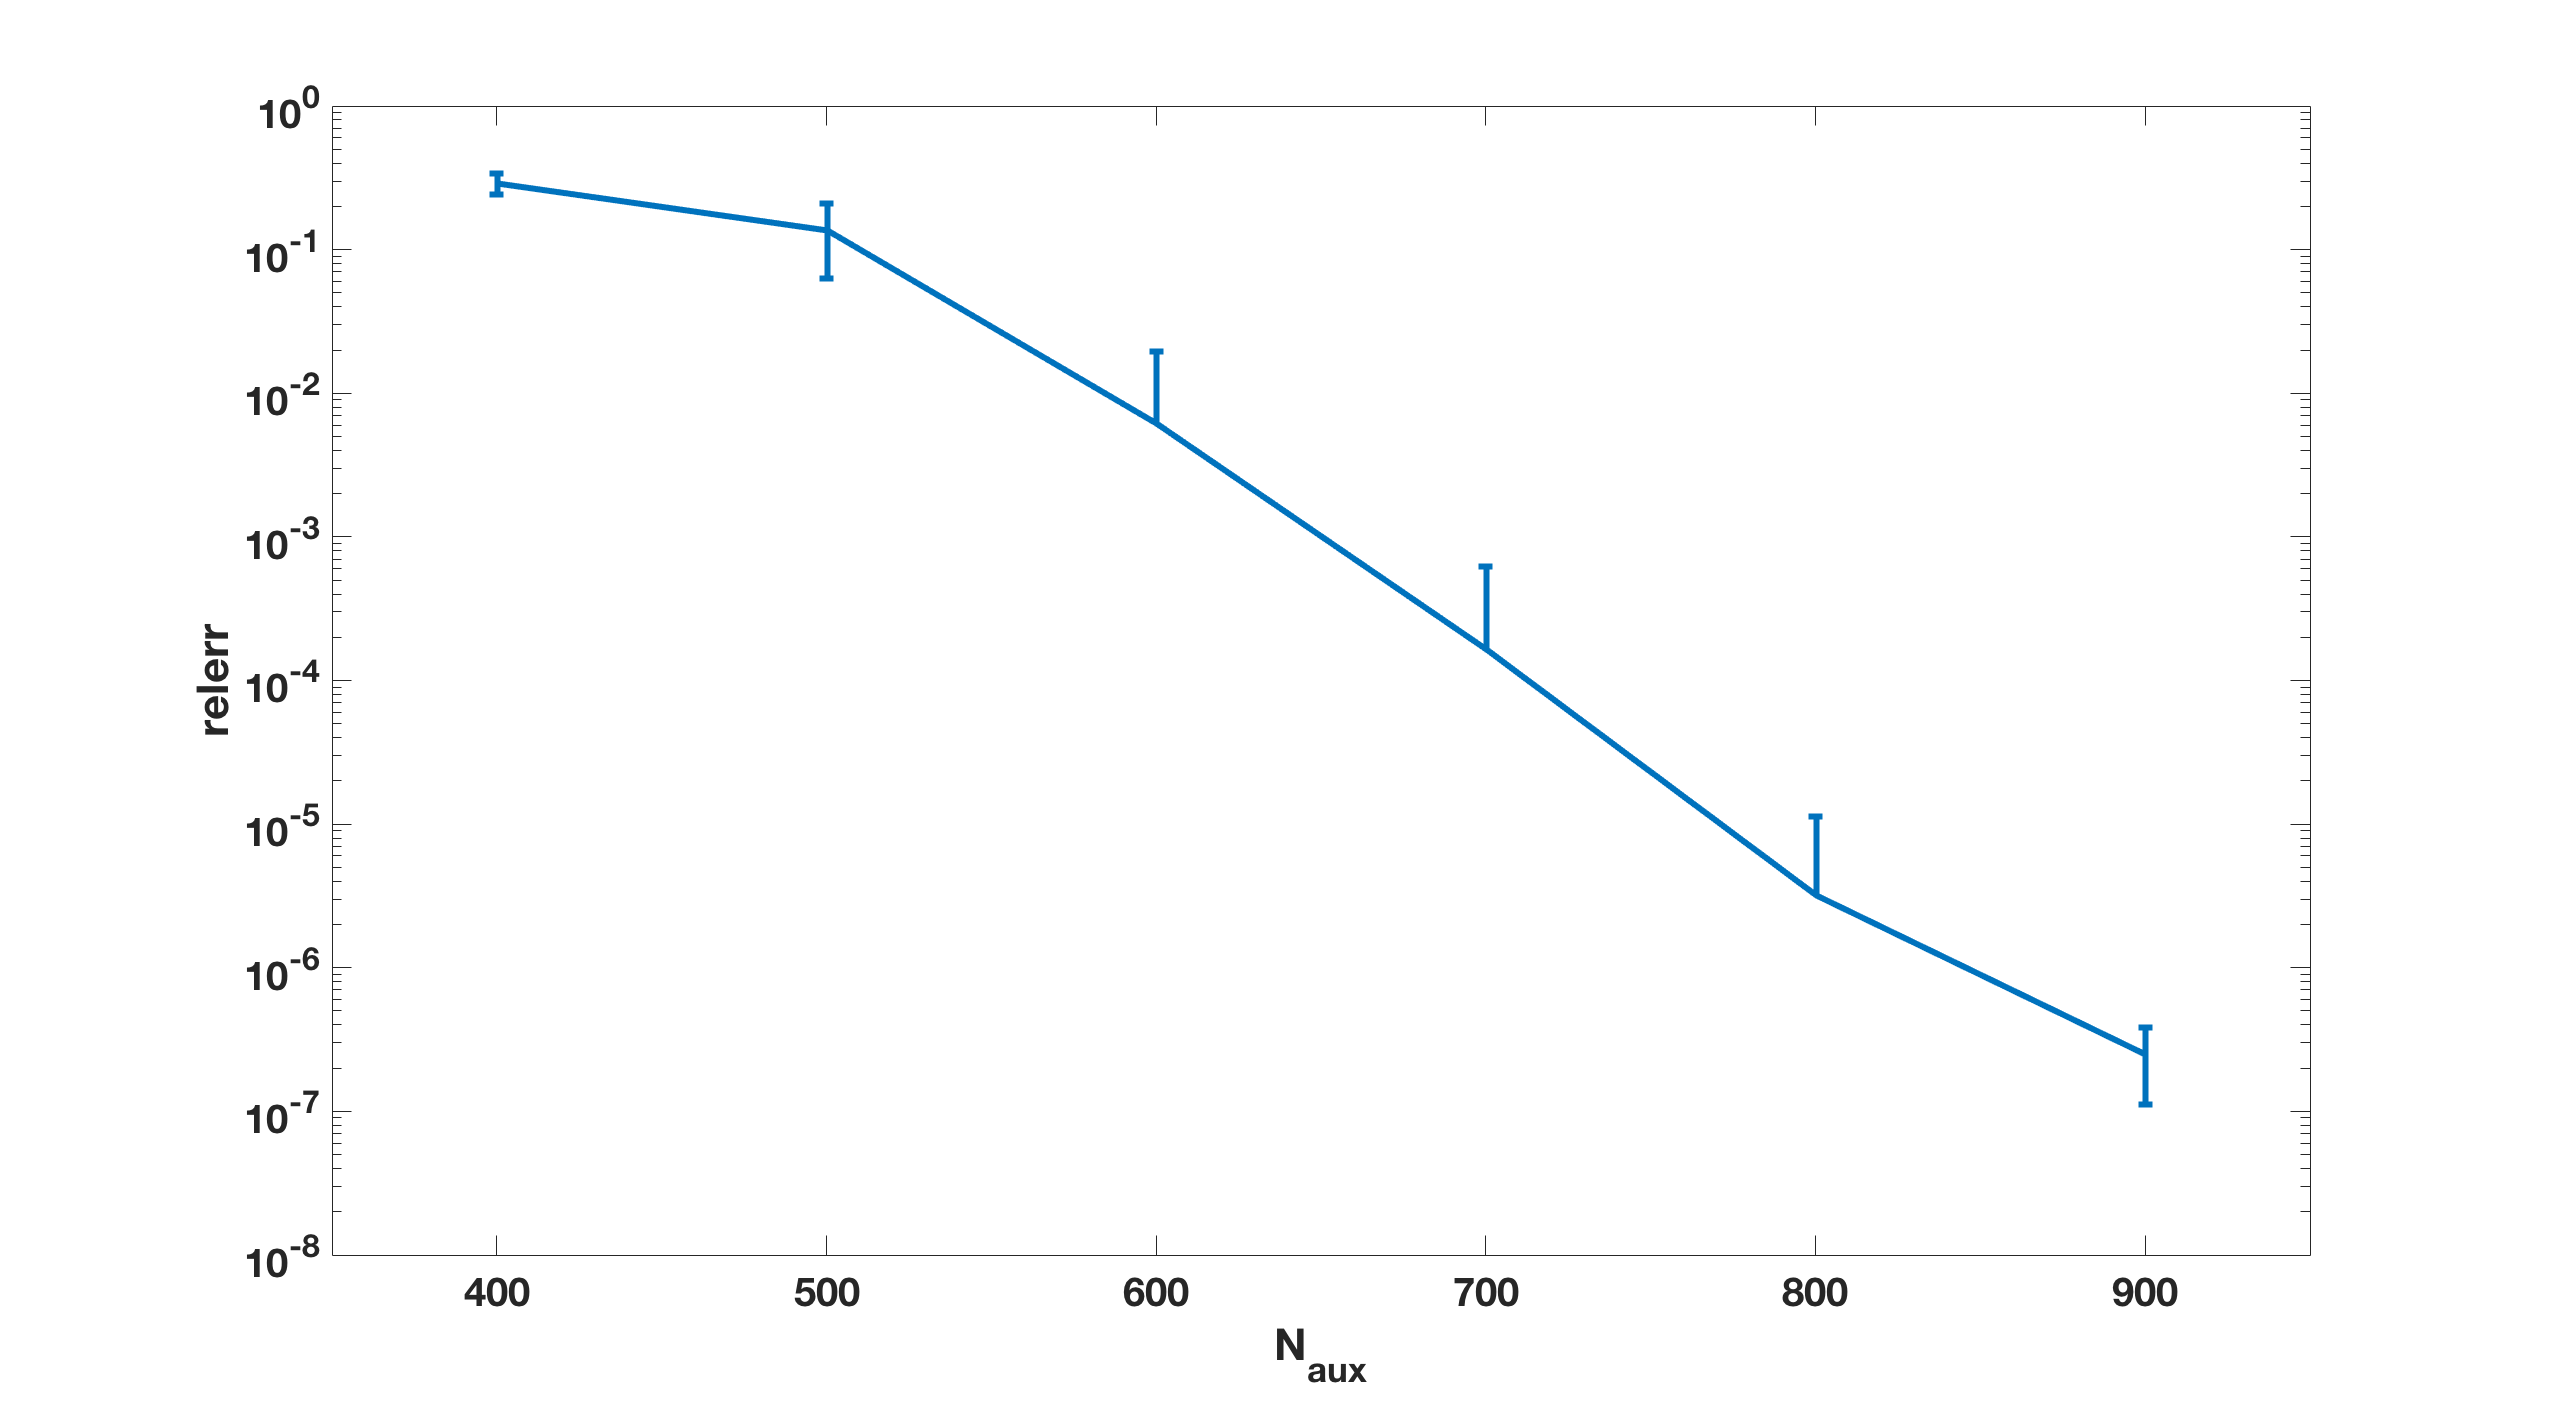
\includegraphics[width = \textwidth]{N200n2048.png}
		\caption{Relative error for different number of interpolation points from $400$ to $900$.}
	\end{subfigure}
	\begin{subfigure}{\textwidth}
		\centering
		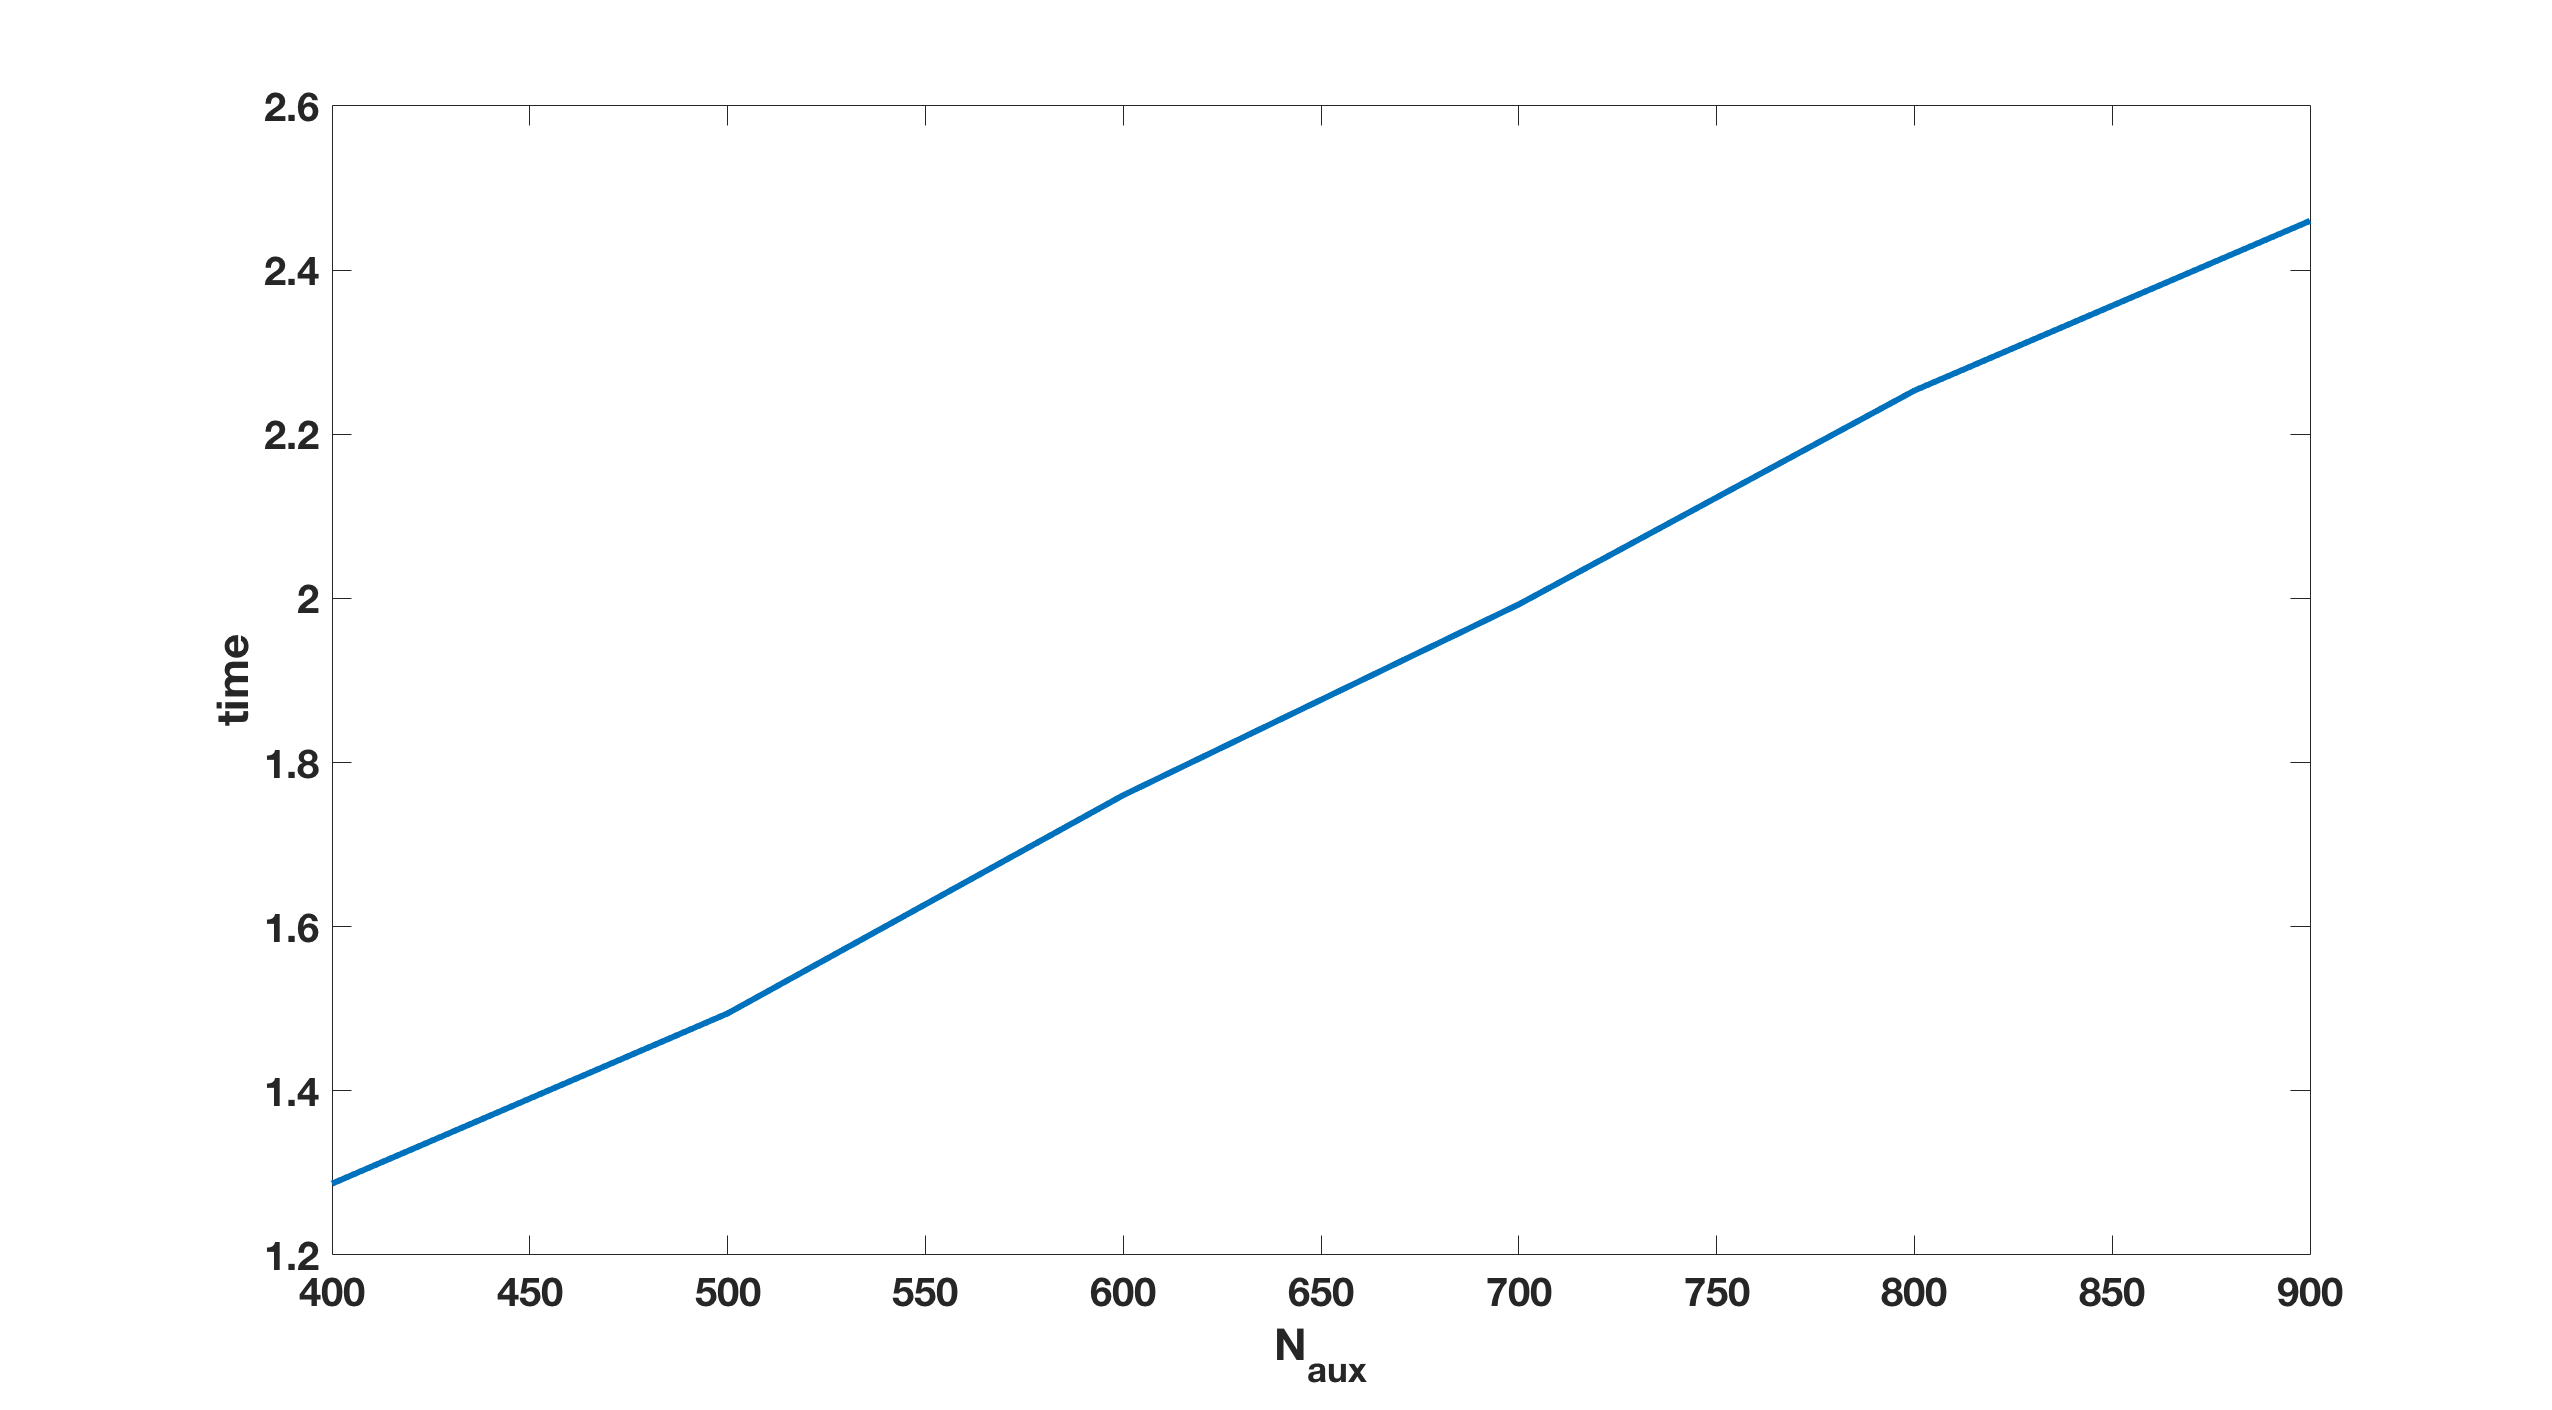
\includegraphics[width = \textwidth]{N200n2048t.png}
		\caption{Run time for different number of interpolation points from $400$ to $900$.}
	\end{subfigure}
\end{figure}



\end{document}